\section{What its parts do}\label{sec:ablations}

DFG v1.3 has many parts (\cref{sec:learner}, \cref{tab:params}). This section asks which of them carry its results. It reports the protocol's 12 ablations (Q5), each DFG alone with one constructor argument changed, and then a post-hoc \emph{core} DFG with nine parts removed at once (\cref{sec:core}). Every run uses the frozen file; only constructor arguments change.

\paragraph{How the runs are compared.} An ablation runs on DFG alone's training sets, column permutations and cross-validation folds, which all come from the fit's random stream. Its $\nstar$ is compared with DFG alone's $\nstar$ computed from the same seeds of DFG alone's own runs. Six ablations (and the core) ran on seeds 0 and 1, six on seed 0 only (\cref{sec:part11}). The ratio is $\log_2(\nstar_{\rm run}/\nstar_{\rm DFG\ alone})$, negative when the run needs less data. A target moves \emph{lower} or \emph{higher} when the ratio is beyond $\mp0.25$; means are over the targets both reach. The five ablation suites hold 65 targets (\code{designed}, \code{dlsymdev}, \code{dlfamdev}, \code{dlheld6}, \code{dlheld7}); only \code{dlheld7} is held out.

\paragraph{Two nulls.} The protocol's null compares DFG alone's seed 1 with its seed 0. Those are different training sets, so it overstates the noise of a paired comparison: it moves 23 of the 65 targets beyond $\pm0.25$. A paired comparison needs a paired null, which was added post hoc: DFG alone refitted on the same training and test sets with another fit stream, so with another column order and other folds and nothing else (\repo{study/part11/interp/ablations/perm_null.py}). The column order is irrelevant to the targets, and no test statistic depends on it, but it can matter through tie-breaking, the block search's orders and the folds. A change that leaves DFG's decisions alone therefore still perturbs its path, and the paired null measures by how much.

\paragraph{Families.} Each target is assigned by hand, from its definition, to one of the nine groups of \cref{sec:interp-atlas} and to three classes (post hoc; \repo{study/part11/interp/ablations/families.py}). \emph{Character targets} are parities, staircases, multiplexers, compositions of parities and majorities and thresholds of a few characters, DNFs, CNFs, decision lists, read-once and random formulas: 71 of the 138 targets, 25 of the 65. \emph{Halfspaces} are majorities and thresholds of a weighted sum, with the dictator, $\mathrm{AND}(x_1,x_2,x_3)$ and an AND of two halfspaces (13 and 7). \emph{Symmetric and mixture targets} are functions of one signed sum, alone or with a parity, a gate, a second sum or an inner term (54 and 33). This class differs from the 54 sum-structured targets of \cref{sec:tasks} by two targets each way: it includes sym8 and sym9, and it counts f7\_01 and fd\_01, thresholds of an unsigned sum, as halfspaces.

\paragraph{Sources.} The summaries are in \repo{study/part11/RESULTS.json} (\texttt{q5\_ablations}, \texttt{q5b\_core}), written by \repo{study/part11/compare_dfg.py}. The groupings, the nulls, the predictions of \cref{sec:abl-test} and the leave-one-in runs of \cref{sec:core} are in \repo{study/part11/interp/ablations/ablations.json}, written by \repo{study/part11/interp/ablations/ablations.py}; the analysis is \repo{study/part11/interp/ablations/ABLATIONS.md}. Models are read from refits of single cells (\repo{study/part11/interp/ablations/refit.py}). A refit uses the instrumented copy of \cref{sec:interp-calib}, so that every feature carries the class that admitted it, and all 36 refits reproduce their run's result file exactly in test error and FLOP count (\repo{study/part11/interp/ablations/results/refits.json}). In four cells the same fit through the evaluation's own loader of the frozen file gives the same model, term by term (\repo{study/part11/interp/ablations/results/refit_crosscheck.json}). The analysis has not been checked by an independent verifier.

% ------------------------------------------------------------------------------------------------------------------
\subsection{Twelve single changes}\label{sec:abl-single}

\begin{table}[t]
\centering{\footnotesize\setlength{\tabcolsep}{2.4pt}\renewcommand{\arraystretch}{1.05}
\begin{tabularx}{\linewidth}{@{}l>{\raggedright\arraybackslash}Xcc>{\raggedright\arraybackslash}p{1.25cm}ccc@{}}
\toprule
run & change & seeds & \hd{all\\(65)} & \hd{newly\\never} & \hd{character\\targets\\(25)} & \hd{halfspaces\\(7)} & \hd{symmetric and\\mixtures\\(33)}\\
\midrule
\code{nosums} & no sum blocks & 0, 1 & \begin{tabular}[t]{@{}c@{}}$+0.91$\\{\scriptsize (2/31) [59]}\end{tabular} & {\scriptsize band11, h6\_01, f7\_08} & \begin{tabular}[t]{@{}c@{}}$+0.16$\\{\scriptsize (1/5) [25]}\end{tabular} & \begin{tabular}[t]{@{}c@{}}$+0.05$\\{\scriptsize (0/1) [7]}\end{tabular} & \begin{tabular}[t]{@{}c@{}}$+1.82$\\{\scriptsize (1/25) [27]}\end{tabular}\\
\code{strict} & stricter tests, $\delta=10^{-4}$ & 0, 1 & \begin{tabular}[t]{@{}c@{}}$+0.06$\\{\scriptsize (9/14) [62]}\end{tabular} & {\scriptsize --} & \begin{tabular}[t]{@{}c@{}}$+0.17$\\{\scriptsize (3/8) [25]}\end{tabular} & \begin{tabular}[t]{@{}c@{}}$-0.23$\\{\scriptsize (4/1) [7]}\end{tabular} & \begin{tabular}[t]{@{}c@{}}$+0.04$\\{\scriptsize (2/5) [30]}\end{tabular}\\
\code{lenient} & more lenient tests, $\delta=0.9$ & 0, 1 & \begin{tabular}[t]{@{}c@{}}$+0.07$\\{\scriptsize (5/13) [62]}\end{tabular} & {\scriptsize --} & \begin{tabular}[t]{@{}c@{}}$+0.12$\\{\scriptsize (2/8) [25]}\end{tabular} & \begin{tabular}[t]{@{}c@{}}$-0.04$\\{\scriptsize (2/1) [7]}\end{tabular} & \begin{tabular}[t]{@{}c@{}}$+0.05$\\{\scriptsize (1/4) [30]}\end{tabular}\\
\code{noeig} & no eigenvector seeds in the block search & 0, 1 & \begin{tabular}[t]{@{}c@{}}$+0.03$\\{\scriptsize (0/1) [62]}\end{tabular} & {\scriptsize --} & \begin{tabular}[t]{@{}c@{}}$+0.00$\\{\scriptsize (0/0) [25]}\end{tabular} & \begin{tabular}[t]{@{}c@{}}$+0.00$\\{\scriptsize (0/0) [7]}\end{tabular} & \begin{tabular}[t]{@{}c@{}}$+0.05$\\{\scriptsize (0/1) [30]}\end{tabular}\\
\code{noblocks} & no linear or spectral block & 0, 1 & \begin{tabular}[t]{@{}c@{}}$-0.02$\\{\scriptsize (6/4) [62]}\end{tabular} & {\scriptsize --} & \begin{tabular}[t]{@{}c@{}}$-0.03$\\{\scriptsize (2/1) [25]}\end{tabular} & \begin{tabular}[t]{@{}c@{}}$-0.19$\\{\scriptsize (3/0) [7]}\end{tabular} & \begin{tabular}[t]{@{}c@{}}$+0.02$\\{\scriptsize (1/3) [30]}\end{tabular}\\
\code{nocomp} & no extension or local classes & 0, 1 & \begin{tabular}[t]{@{}c@{}}$+0.00$\\{\scriptsize (2/2) [62]}\end{tabular} & {\scriptsize --} & \begin{tabular}[t]{@{}c@{}}$+0.02$\\{\scriptsize (1/2) [25]}\end{tabular} & \begin{tabular}[t]{@{}c@{}}$+0.00$\\{\scriptsize (0/0) [7]}\end{tabular} & \begin{tabular}[t]{@{}c@{}}$-0.02$\\{\scriptsize (1/0) [30]}\end{tabular}\\
\code{noweighted} & no weighted blocks & 0 & \begin{tabular}[t]{@{}c@{}}$+0.02$\\{\scriptsize (0/1) [62]}\end{tabular} & {\scriptsize --} & \begin{tabular}[t]{@{}c@{}}$+0.01$\\{\scriptsize (0/0) [25]}\end{tabular} & \begin{tabular}[t]{@{}c@{}}$+0.00$\\{\scriptsize (0/0) [7]}\end{tabular} & \begin{tabular}[t]{@{}c@{}}$+0.03$\\{\scriptsize (0/1) [30]}\end{tabular}\\
\code{nosmalln} & no forced variant, no cross-validation & 0 & \begin{tabular}[t]{@{}c@{}}$+0.12$\\{\scriptsize (0/10) [62]}\end{tabular} & {\scriptsize --} & \begin{tabular}[t]{@{}c@{}}$+0.22$\\{\scriptsize (0/8) [25]}\end{tabular} & \begin{tabular}[t]{@{}c@{}}$-0.03$\\{\scriptsize (0/0) [7]}\end{tabular} & \begin{tabular}[t]{@{}c@{}}$+0.07$\\{\scriptsize (0/2) [30]}\end{tabular}\\
\code{nobg} & no kernel background & 0 & \begin{tabular}[t]{@{}c@{}}$-0.10$\\{\scriptsize (7/3) [62]}\end{tabular} & {\scriptsize --} & \begin{tabular}[t]{@{}c@{}}$-0.07$\\{\scriptsize (3/2) [25]}\end{tabular} & \begin{tabular}[t]{@{}c@{}}$-0.09$\\{\scriptsize (1/0) [7]}\end{tabular} & \begin{tabular}[t]{@{}c@{}}$-0.12$\\{\scriptsize (3/1) [30]}\end{tabular}\\
\code{lsread} & least-squares readout & 0 & \begin{tabular}[t]{@{}c@{}}$-0.01$\\{\scriptsize (2/1) [62]}\end{tabular} & {\scriptsize --} & \begin{tabular}[t]{@{}c@{}}$-0.01$\\{\scriptsize (2/1) [25]}\end{tabular} & \begin{tabular}[t]{@{}c@{}}$+0.00$\\{\scriptsize (0/0) [7]}\end{tabular} & \begin{tabular}[t]{@{}c@{}}$-0.02$\\{\scriptsize (0/0) [30]}\end{tabular}\\
\code{K3} & global search to degree 3 & 0 & \begin{tabular}[t]{@{}c@{}}$+0.02$\\{\scriptsize (2/1) [62]}\end{tabular} & {\scriptsize --} & \begin{tabular}[t]{@{}c@{}}$+0.08$\\{\scriptsize (1/1) [25]}\end{tabular} & \begin{tabular}[t]{@{}c@{}}$-0.05$\\{\scriptsize (1/0) [7]}\end{tabular} & \begin{tabular}[t]{@{}c@{}}$-0.01$\\{\scriptsize (0/0) [30]}\end{tabular}\\
\code{labelnoise} & tests scaled to the labels' noise & 0 & \begin{tabular}[t]{@{}c@{}}$+0.14$\\{\scriptsize (5/15) [62]}\end{tabular} & {\scriptsize --} & \begin{tabular}[t]{@{}c@{}}$+0.23$\\{\scriptsize (2/9) [25]}\end{tabular} & \begin{tabular}[t]{@{}c@{}}$-0.17$\\{\scriptsize (2/0) [7]}\end{tabular} & \begin{tabular}[t]{@{}c@{}}$+0.14$\\{\scriptsize (1/6) [30]}\end{tabular}\\
\midrule
paired null & other column order and folds, same training sets & 0 & \begin{tabular}[t]{@{}c@{}}$+0.00$\\{\scriptsize (0/1) [62]}\end{tabular} & {\scriptsize --} & \begin{tabular}[t]{@{}c@{}}$+0.00$\\{\scriptsize (0/1) [25]}\end{tabular} & \begin{tabular}[t]{@{}c@{}}$+0.00$\\{\scriptsize (0/0) [7]}\end{tabular} & \begin{tabular}[t]{@{}c@{}}$-0.00$\\{\scriptsize (0/0) [30]}\end{tabular}\\
paired null & other column order and folds, same training sets & 0, 1 & \begin{tabular}[t]{@{}c@{}}$-0.02$\\{\scriptsize (2/1) [62]}\end{tabular} & {\scriptsize --} & \begin{tabular}[t]{@{}c@{}}$-0.02$\\{\scriptsize (1/0) [25]}\end{tabular} & \begin{tabular}[t]{@{}c@{}}$+0.00$\\{\scriptsize (0/0) [7]}\end{tabular} & \begin{tabular}[t]{@{}c@{}}$-0.02$\\{\scriptsize (1/1) [30]}\end{tabular}\\
unpaired null & seed 1 against seed 0: other training sets & 1 vs 0 & \begin{tabular}[t]{@{}c@{}}$-0.04$\\{\scriptsize (13/10) [62]}\end{tabular} & {\scriptsize --} & \begin{tabular}[t]{@{}c@{}}$-0.02$\\{\scriptsize (5/4) [25]}\end{tabular} & \begin{tabular}[t]{@{}c@{}}$-0.17$\\{\scriptsize (2/1) [7]}\end{tabular} & \begin{tabular}[t]{@{}c@{}}$-0.04$\\{\scriptsize (6/5) [30]}\end{tabular}\\
\bottomrule
\end{tabularx}
}
\caption{The 12 ablations of Q5 on the 65 targets of the five ablation suites, against DFG alone on the same seeds and training sets \status{Numerical}. Each cell gives the mean $\log_2$ ratio of the run's $\nstar$ to DFG alone's over the targets both learn; below it, the targets on which the run needs clearly less / clearly more data (beyond $\mp0.25$, or only one reaches 10\% error), and in brackets the number both learn. ``Newly never'': targets the run never brings to 10\% error by $n=16384$ while DFG alone does. Class sizes in the header (\cref{sec:ablations}, ``Families''). The three targets that DFG alone never learns (fd\_10, h6\_00, f7\_05) are in no mean. Bottom: the paired null (post hoc), DFG alone refitted on the same training sets with another column order and other cross-validation folds, and the protocol's unpaired null. Sources: \repo{study/part11/RESULTS.json} (\texttt{q5\_ablations}; the pooled column is checked against it) and \repo{study/part11/interp/ablations/ablations.json} via \repo{paper_dfg/make_tables.py}.}
\label{tab:ablations}
\end{table}

\begin{figure}[t]
\centering
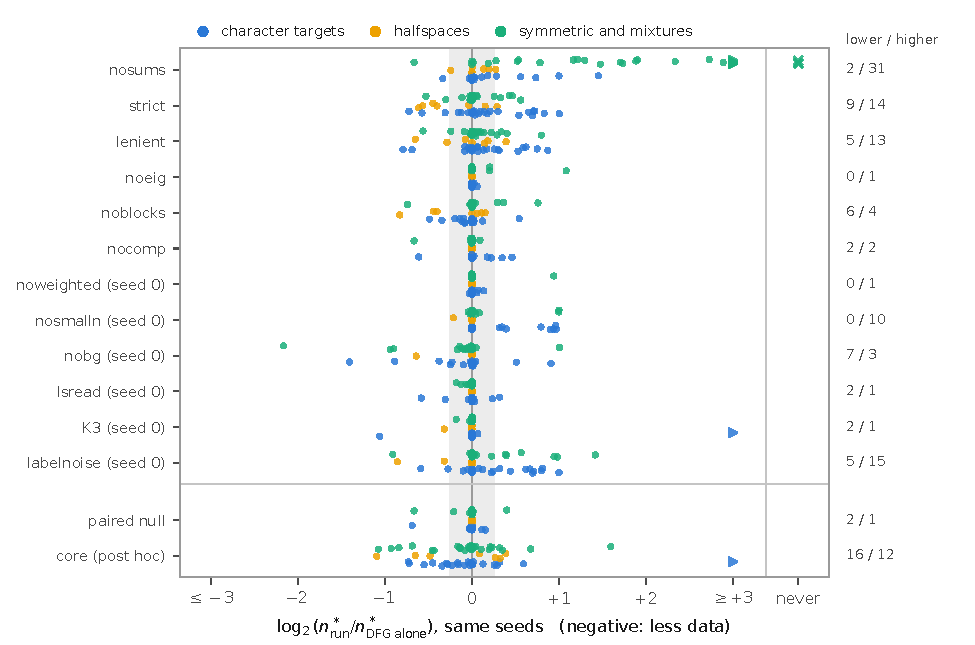
\includegraphics[width=\linewidth]{figures/fig_ablations.pdf}
\caption{Every target of the five ablation suites, one row per run: the $\log_2$ ratio of the run's $\nstar$ to DFG alone's on the same seeds \status{Numerical}. Colour gives the target's class; the grey band is the tie band $\pm0.25$. Ratios beyond $\pm3$ are drawn at the edge (triangles), and ``never'' (the run never reaches 10\% error where DFG alone does) in the right-hand column. Right: the numbers of targets clearly lower / clearly higher. Bottom: the paired null on seeds 0 and 1 (post hoc) and the core DFG of \cref{sec:core} on the same 65 targets (post hoc). Source: \repo{study/part11/interp/ablations/ablations.json} via \repo{paper_dfg/make_figures.py}; the plotted points are in \repo{paper_dfg/figures/fig_ablations.json}.}
\label{fig:ablations}
\end{figure}

\begin{table}[t]
\centering{\footnotesize\setlength{\tabcolsep}{3pt}\renewcommand{\arraystretch}{1.05}
\begin{tabular}{@{}lcccccccc@{}}
\toprule
run & \hd{parities\\(3)} & \hd{stair-\\cases\\(1)} & \hd{half-\\spaces\\(7)} & \hd{compo-\\sitions\\(6)} & \hd{formulas\\(11)} & \hd{random\\formulas\\(4)} & \hd{sym-\\metric\\(12)} & \hd{mixtures\\(21)}\\
\midrule
\code{nosums} & \begin{tabular}[t]{@{}c@{}}$+0.00$\\{\scriptsize (0/0)}\end{tabular} & \begin{tabular}[t]{@{}c@{}}$+0.00$\\{\scriptsize (0/0)}\end{tabular} & \begin{tabular}[t]{@{}c@{}}$+0.05$\\{\scriptsize (0/1)}\end{tabular} & \begin{tabular}[t]{@{}c@{}}$+0.11$\\{\scriptsize (1/1)}\end{tabular} & \begin{tabular}[t]{@{}c@{}}$+0.17$\\{\scriptsize (0/3)}\end{tabular} & \begin{tabular}[t]{@{}c@{}}$+0.36$\\{\scriptsize (0/1)}\end{tabular} & \begin{tabular}[t]{@{}c@{}}$+2.78$\\{\scriptsize (0/9)}\end{tabular} & \begin{tabular}[t]{@{}c@{}}$+1.54$\\{\scriptsize (1/16)}\end{tabular}\\
\code{strict} & \begin{tabular}[t]{@{}c@{}}$+0.40$\\{\scriptsize (0/1)}\end{tabular} & \begin{tabular}[t]{@{}c@{}}$+0.83$\\{\scriptsize (0/1)}\end{tabular} & \begin{tabular}[t]{@{}c@{}}$-0.23$\\{\scriptsize (4/1)}\end{tabular} & \begin{tabular}[t]{@{}c@{}}$+0.09$\\{\scriptsize (2/2)}\end{tabular} & \begin{tabular}[t]{@{}c@{}}$+0.01$\\{\scriptsize (1/2)}\end{tabular} & \begin{tabular}[t]{@{}c@{}}$+0.39$\\{\scriptsize (0/2)}\end{tabular} & \begin{tabular}[t]{@{}c@{}}$-0.01$\\{\scriptsize (0/0)}\end{tabular} & \begin{tabular}[t]{@{}c@{}}$+0.06$\\{\scriptsize (2/5)}\end{tabular}\\
\code{lenient} & \begin{tabular}[t]{@{}c@{}}$-0.26$\\{\scriptsize (1/0)}\end{tabular} & \begin{tabular}[t]{@{}c@{}}$+0.00$\\{\scriptsize (0/0)}\end{tabular} & \begin{tabular}[t]{@{}c@{}}$-0.04$\\{\scriptsize (2/1)}\end{tabular} & \begin{tabular}[t]{@{}c@{}}$+0.36$\\{\scriptsize (0/3)}\end{tabular} & \begin{tabular}[t]{@{}c@{}}$+0.19$\\{\scriptsize (0/5)}\end{tabular} & \begin{tabular}[t]{@{}c@{}}$-0.11$\\{\scriptsize (1/0)}\end{tabular} & \begin{tabular}[t]{@{}c@{}}$+0.07$\\{\scriptsize (0/1)}\end{tabular} & \begin{tabular}[t]{@{}c@{}}$+0.05$\\{\scriptsize (1/3)}\end{tabular}\\
\code{noeig} & \begin{tabular}[t]{@{}c@{}}$+0.00$\\{\scriptsize (0/0)}\end{tabular} & \begin{tabular}[t]{@{}c@{}}$+0.00$\\{\scriptsize (0/0)}\end{tabular} & \begin{tabular}[t]{@{}c@{}}$+0.00$\\{\scriptsize (0/0)}\end{tabular} & \begin{tabular}[t]{@{}c@{}}$+0.00$\\{\scriptsize (0/0)}\end{tabular} & \begin{tabular}[t]{@{}c@{}}$+0.01$\\{\scriptsize (0/0)}\end{tabular} & \begin{tabular}[t]{@{}c@{}}$-0.00$\\{\scriptsize (0/0)}\end{tabular} & \begin{tabular}[t]{@{}c@{}}$+0.02$\\{\scriptsize (0/0)}\end{tabular} & \begin{tabular}[t]{@{}c@{}}$+0.06$\\{\scriptsize (0/1)}\end{tabular}\\
\code{noblocks} & \begin{tabular}[t]{@{}c@{}}$+0.00$\\{\scriptsize (0/0)}\end{tabular} & \begin{tabular}[t]{@{}c@{}}$+0.00$\\{\scriptsize (0/0)}\end{tabular} & \begin{tabular}[t]{@{}c@{}}$-0.19$\\{\scriptsize (3/0)}\end{tabular} & \begin{tabular}[t]{@{}c@{}}$-0.07$\\{\scriptsize (1/0)}\end{tabular} & \begin{tabular}[t]{@{}c@{}}$+0.01$\\{\scriptsize (0/1)}\end{tabular} & \begin{tabular}[t]{@{}c@{}}$-0.12$\\{\scriptsize (1/0)}\end{tabular} & \begin{tabular}[t]{@{}c@{}}$-0.00$\\{\scriptsize (0/0)}\end{tabular} & \begin{tabular}[t]{@{}c@{}}$+0.04$\\{\scriptsize (1/3)}\end{tabular}\\
\code{nocomp} & \begin{tabular}[t]{@{}c@{}}$+0.00$\\{\scriptsize (0/0)}\end{tabular} & \begin{tabular}[t]{@{}c@{}}$+0.00$\\{\scriptsize (0/0)}\end{tabular} & \begin{tabular}[t]{@{}c@{}}$+0.00$\\{\scriptsize (0/0)}\end{tabular} & \begin{tabular}[t]{@{}c@{}}$-0.07$\\{\scriptsize (1/0)}\end{tabular} & \begin{tabular}[t]{@{}c@{}}$+0.08$\\{\scriptsize (0/2)}\end{tabular} & \begin{tabular}[t]{@{}c@{}}$+0.05$\\{\scriptsize (0/0)}\end{tabular} & \begin{tabular}[t]{@{}c@{}}$+0.00$\\{\scriptsize (0/0)}\end{tabular} & \begin{tabular}[t]{@{}c@{}}$-0.03$\\{\scriptsize (1/0)}\end{tabular}\\
\code{noweighted} & \begin{tabular}[t]{@{}c@{}}$+0.00$\\{\scriptsize (0/0)}\end{tabular} & \begin{tabular}[t]{@{}c@{}}$+0.00$\\{\scriptsize (0/0)}\end{tabular} & \begin{tabular}[t]{@{}c@{}}$+0.00$\\{\scriptsize (0/0)}\end{tabular} & \begin{tabular}[t]{@{}c@{}}$+0.00$\\{\scriptsize (0/0)}\end{tabular} & \begin{tabular}[t]{@{}c@{}}$+0.02$\\{\scriptsize (0/0)}\end{tabular} & \begin{tabular}[t]{@{}c@{}}$+0.00$\\{\scriptsize (0/0)}\end{tabular} & \begin{tabular}[t]{@{}c@{}}$+0.00$\\{\scriptsize (0/0)}\end{tabular} & \begin{tabular}[t]{@{}c@{}}$+0.04$\\{\scriptsize (0/1)}\end{tabular}\\
\code{nosmalln} & \begin{tabular}[t]{@{}c@{}}$+0.26$\\{\scriptsize (0/1)}\end{tabular} & \begin{tabular}[t]{@{}c@{}}$+0.00$\\{\scriptsize (0/0)}\end{tabular} & \begin{tabular}[t]{@{}c@{}}$-0.03$\\{\scriptsize (0/0)}\end{tabular} & \begin{tabular}[t]{@{}c@{}}$+0.38$\\{\scriptsize (0/3)}\end{tabular} & \begin{tabular}[t]{@{}c@{}}$+0.15$\\{\scriptsize (0/3)}\end{tabular} & \begin{tabular}[t]{@{}c@{}}$+0.22$\\{\scriptsize (0/1)}\end{tabular} & \begin{tabular}[t]{@{}c@{}}$+0.11$\\{\scriptsize (0/1)}\end{tabular} & \begin{tabular}[t]{@{}c@{}}$+0.05$\\{\scriptsize (0/1)}\end{tabular}\\
\code{nobg} & \begin{tabular}[t]{@{}c@{}}$+0.00$\\{\scriptsize (0/0)}\end{tabular} & \begin{tabular}[t]{@{}c@{}}$+0.04$\\{\scriptsize (0/0)}\end{tabular} & \begin{tabular}[t]{@{}c@{}}$-0.09$\\{\scriptsize (1/0)}\end{tabular} & \begin{tabular}[t]{@{}c@{}}$-0.12$\\{\scriptsize (1/0)}\end{tabular} & \begin{tabular}[t]{@{}c@{}}$-0.10$\\{\scriptsize (1/1)}\end{tabular} & \begin{tabular}[t]{@{}c@{}}$+0.00$\\{\scriptsize (1/1)}\end{tabular} & \begin{tabular}[t]{@{}c@{}}$-0.04$\\{\scriptsize (0/0)}\end{tabular} & \begin{tabular}[t]{@{}c@{}}$-0.16$\\{\scriptsize (3/1)}\end{tabular}\\
\code{lsread} & \begin{tabular}[t]{@{}c@{}}$+0.00$\\{\scriptsize (0/0)}\end{tabular} & \begin{tabular}[t]{@{}c@{}}$+0.00$\\{\scriptsize (0/0)}\end{tabular} & \begin{tabular}[t]{@{}c@{}}$+0.00$\\{\scriptsize (0/0)}\end{tabular} & \begin{tabular}[t]{@{}c@{}}$+0.06$\\{\scriptsize (0/1)}\end{tabular} & \begin{tabular}[t]{@{}c@{}}$-0.06$\\{\scriptsize (2/0)}\end{tabular} & \begin{tabular}[t]{@{}c@{}}$-0.01$\\{\scriptsize (0/0)}\end{tabular} & \begin{tabular}[t]{@{}c@{}}$-0.00$\\{\scriptsize (0/0)}\end{tabular} & \begin{tabular}[t]{@{}c@{}}$-0.02$\\{\scriptsize (0/0)}\end{tabular}\\
\code{K3} & \begin{tabular}[t]{@{}c@{}}$+1.00$\\{\scriptsize (0/1)}\end{tabular} & \begin{tabular}[t]{@{}c@{}}$+0.07$\\{\scriptsize (0/0)}\end{tabular} & \begin{tabular}[t]{@{}c@{}}$-0.05$\\{\scriptsize (1/0)}\end{tabular} & \begin{tabular}[t]{@{}c@{}}$+0.00$\\{\scriptsize (0/0)}\end{tabular} & \begin{tabular}[t]{@{}c@{}}$-0.00$\\{\scriptsize (0/0)}\end{tabular} & \begin{tabular}[t]{@{}c@{}}$-0.26$\\{\scriptsize (1/0)}\end{tabular} & \begin{tabular}[t]{@{}c@{}}$+0.00$\\{\scriptsize (0/0)}\end{tabular} & \begin{tabular}[t]{@{}c@{}}$-0.01$\\{\scriptsize (0/0)}\end{tabular}\\
\code{labelnoise} & \begin{tabular}[t]{@{}c@{}}$+0.00$\\{\scriptsize (0/0)}\end{tabular} & \begin{tabular}[t]{@{}c@{}}$+0.70$\\{\scriptsize (0/1)}\end{tabular} & \begin{tabular}[t]{@{}c@{}}$-0.17$\\{\scriptsize (2/0)}\end{tabular} & \begin{tabular}[t]{@{}c@{}}$+0.11$\\{\scriptsize (1/1)}\end{tabular} & \begin{tabular}[t]{@{}c@{}}$+0.33$\\{\scriptsize (1/6)}\end{tabular} & \begin{tabular}[t]{@{}c@{}}$+0.19$\\{\scriptsize (0/1)}\end{tabular} & \begin{tabular}[t]{@{}c@{}}$+0.10$\\{\scriptsize (0/1)}\end{tabular} & \begin{tabular}[t]{@{}c@{}}$+0.15$\\{\scriptsize (1/5)}\end{tabular}\\
\midrule
paired null (0, 1) & \begin{tabular}[t]{@{}c@{}}$-0.00$\\{\scriptsize (0/0)}\end{tabular} & \begin{tabular}[t]{@{}c@{}}$+0.00$\\{\scriptsize (0/0)}\end{tabular} & \begin{tabular}[t]{@{}c@{}}$+0.00$\\{\scriptsize (0/0)}\end{tabular} & \begin{tabular}[t]{@{}c@{}}$-0.11$\\{\scriptsize (1/0)}\end{tabular} & \begin{tabular}[t]{@{}c@{}}$+0.02$\\{\scriptsize (0/0)}\end{tabular} & \begin{tabular}[t]{@{}c@{}}$-0.00$\\{\scriptsize (0/0)}\end{tabular} & \begin{tabular}[t]{@{}c@{}}$-0.02$\\{\scriptsize (0/0)}\end{tabular} & \begin{tabular}[t]{@{}c@{}}$-0.01$\\{\scriptsize (1/1)}\end{tabular}\\
paired null (0) & \begin{tabular}[t]{@{}c@{}}$-0.00$\\{\scriptsize (0/0)}\end{tabular} & \begin{tabular}[t]{@{}c@{}}$+0.00$\\{\scriptsize (0/0)}\end{tabular} & \begin{tabular}[t]{@{}c@{}}$+0.00$\\{\scriptsize (0/0)}\end{tabular} & \begin{tabular}[t]{@{}c@{}}$-0.02$\\{\scriptsize (0/0)}\end{tabular} & \begin{tabular}[t]{@{}c@{}}$+0.02$\\{\scriptsize (0/1)}\end{tabular} & \begin{tabular}[t]{@{}c@{}}$-0.00$\\{\scriptsize (0/0)}\end{tabular} & \begin{tabular}[t]{@{}c@{}}$+0.00$\\{\scriptsize (0/0)}\end{tabular} & \begin{tabular}[t]{@{}c@{}}$-0.00$\\{\scriptsize (0/0)}\end{tabular}\\
unpaired null & \begin{tabular}[t]{@{}c@{}}$-0.33$\\{\scriptsize (1/0)}\end{tabular} & \begin{tabular}[t]{@{}c@{}}$+0.01$\\{\scriptsize (0/0)}\end{tabular} & \begin{tabular}[t]{@{}c@{}}$-0.17$\\{\scriptsize (2/1)}\end{tabular} & \begin{tabular}[t]{@{}c@{}}$+0.17$\\{\scriptsize (1/2)}\end{tabular} & \begin{tabular}[t]{@{}c@{}}$-0.01$\\{\scriptsize (2/1)}\end{tabular} & \begin{tabular}[t]{@{}c@{}}$-0.07$\\{\scriptsize (1/1)}\end{tabular} & \begin{tabular}[t]{@{}c@{}}$+0.01$\\{\scriptsize (1/1)}\end{tabular} & \begin{tabular}[t]{@{}c@{}}$-0.06$\\{\scriptsize (5/4)}\end{tabular}\\
\midrule
core (post hoc) & \begin{tabular}[t]{@{}c@{}}$+2.01$\\{\scriptsize (0/1)}\end{tabular} & \begin{tabular}[t]{@{}c@{}}$-0.08$\\{\scriptsize (0/0)}\end{tabular} & \begin{tabular}[t]{@{}c@{}}$-0.17$\\{\scriptsize (3/3)}\end{tabular} & \begin{tabular}[t]{@{}c@{}}$-0.15$\\{\scriptsize (3/1)}\end{tabular} & \begin{tabular}[t]{@{}c@{}}$-0.04$\\{\scriptsize (2/2)}\end{tabular} & \begin{tabular}[t]{@{}c@{}}$-0.27$\\{\scriptsize (2/1)}\end{tabular} & \begin{tabular}[t]{@{}c@{}}$-0.03$\\{\scriptsize (0/0)}\end{tabular} & \begin{tabular}[t]{@{}c@{}}$-0.05$\\{\scriptsize (6/4)}\end{tabular}\\
\bottomrule
\end{tabular}
}
\caption{The ablations by target family (the groups of \cref{sec:interp-atlas}; group sizes in the header) on the 65 targets of the five ablation suites \status{Numerical; families post hoc}. Each cell: mean $\log_2$ ratio over the targets both learn, and the targets clearly lower / clearly higher. The symmetric group holds the three targets no learner learns, so its means are over 9 targets (6 under \code{nosums}). Bottom: the paired and unpaired nulls, and the core DFG on the same 65 targets (post hoc). Source: \repo{study/part11/interp/ablations/ablations.json}.}
\label{tab:abl-family}
\end{table}

\Cref{tab:ablations,tab:abl-family} and \cref{fig:ablations} give the results.

\paragraph{The paired null} \status{Numerical; post hoc}. On seed 0 the re-permuted fits move 1 of the 65 targets beyond $\pm0.25$ (dlist5, $+0.39$), and 10 of the 65 ratios are not zero; the mean $|\text{ratio}|$ is 0.012. On seeds 0 and 1 they move 3 (andxor $-0.69$, thrsum $-0.66$, h6\_07 $+0.40$), with mean $|\text{ratio}|$ 0.038. Over all 138 targets of the 11 suites they move 8 on seeds 0 and 1 (mean $|\text{ratio}|$ 0.040). The unpaired null moves 23 to 31 of the 65 targets, depending on the pair of seeds.

\paragraph{What carries the results} \status{Numerical}.
\begin{itemize}
\item \emph{Sum blocks.} Without them (\code{nosums}) the mean ratio is $+0.91$ over the 59 targets both learn, with 31 clearly higher and 2 lower, and DFG no longer learns band11, h6\_01 and f7\_08. The cost falls on the symmetric targets ($+2.78$, 9 of the 9 that DFG alone learns move, 3 of them to ``never'') and the mixtures ($+1.54$, 16 of 21 higher). Character targets lose little ($+0.16$; rand3, parmaj, h6\_05, fd\_07 and dnf3 move up). They are of the kinds the atlas found encoded in part by blocks before their characters are all detectable: parmaj by two folded blocks, formulas by the blocks of a clause or term (\cref{sec:interp-atlas}). The two seeds agree: 27 targets move up on both and none in opposite directions.
\item \emph{Tests scaled to the residual} (\code{labelnoise}, $+0.14$; 15 higher, 5 lower) and \emph{the small-$n$ machinery} (\code{nosmalln}, $+0.12$; 10 higher, none lower) come next, mostly on character targets (\cref{sec:abl-smalln,sec:abl-label}).
\end{itemize}

\paragraph{What moves both ways} \status{Numerical}. The two test levels, the kernel background and the linear and spectral blocks move 10 to 23 targets each, in both directions, with means between $-0.10$ and $+0.07$. Halfspaces gain from \code{strict} ($-0.23$), \code{noblocks} ($-0.19$) and \code{labelnoise} ($-0.17$), three changes that keep features out of the model at small $n$ (\cref{sec:abl-test}). For \code{strict} and \code{lenient}, most movements are one grid step on one seed: 24 and 22 targets move on one seed only, 5 and 4 on both.

\paragraph{What can be removed} \status{Numerical}. Five parts stay within the paired null, or close to it, on these 65 targets:
\begin{itemize}
\item the eigenvector seeds of the block search (\code{noeig}): 1 target moves, h6\_10 ($+1.08$);
\item the extension and local classes (\code{nocomp}): 4 move, among them andxor and thrsum, which the paired null also moves by as much;
\item the weighted blocks (\code{noweighted}): 1 moves, h6\_10 again ($+0.94$), the target they were designed after (\cref{tab:status});
\item the logistic refinement (\code{lsread}): 3 move, by at most 0.58;
\item the search of degrees 4--6 (\code{K3}): 3 move, of which only par4 by much ($+3.01$; \cref{sec:abl-k3}).
\end{itemize}
Their mean $|\text{ratio}|$ is 0.020--0.075, against 0.012 and 0.038 for the paired null on one and two seeds.

\emph{Reading} \status{Heuristic}. On these suites DFG's results come from the sum blocks, with the residual scaling of the tests and the small-$n$ machinery as smaller contributors. Five parts can each be removed without a change larger than an arbitrary perturbation of the path produces. Two qualifications apply. The suites contain few targets that need those parts: one pure 4-parity, no dense halfspace on more than 13 inputs, no degree-5 parity. And the parts are removed one at a time, so they may substitute for one another. \Cref{sec:core} removes them together.

% ------------------------------------------------------------------------------------------------------------------
\subsection{The test or the search}\label{sec:abl-test}

\code{strict} ($\delta=10^{-4}$) and \code{lenient} ($\delta=0.9$) move the log term of every test by $+6.91$ and $-2.20$ nats. If a target's data cost is set by a test, its $\nstar$ should move by a predictable amount; if it is set by the search, it should not move. \Cref{sec:interp-when} goes through these two runs target by target (\cref{fig:dyn-when}); this subsection summarizes them and adds the refits behind the asymmetry between the two.

\paragraph{Parities: the test, exactly} \status{Numerical}. By \cref{prop:parity}, a $k$-parity passes round 0's test exactly when $n(1-\bar y^2)>n_{\rm thr}(k,d)$, and $n_{\rm thr}$ moves by $+13.8$ and $-4.4$ rows with $\delta$. At $d=30$ it moves from 22.3, 26.8 and 30.6 ($k=2,3,4$) to 36.1, 40.6 and 44.4 under \code{strict}, and to 17.9, 22.4 and 26.2 under \code{lenient}. Applied seed by seed to each training set's own $\bar y$, this predicts the measured changes of $\nstar$ to within 0.03: par3 $+0.98$ against $+1.00$ under \code{strict}, and 0 against 0 under \code{lenient}; par4 $+0.20$ against $+0.21$, and $-0.79$ against $-0.79$. par2 moves under neither, because the forced variant fits it at $n=16$, below every $n_{\rm thr}$ here, and the cross-validation's choice does not depend on $\delta$.

\paragraph{Other character targets} \status{Numerical}. By \cref{prop:nglob}(b), $n_{\rm glob}$ is proportional to the log term, so \code{strict} should raise it by $+0.54$ to $+0.86$ doublings (degree 4 to degree 1), and \code{lenient} lower it by $-0.22$ to $-0.43$. \code{strict} raises $\nstar$ beyond 0.25 on 8 of the 25 character targets (par3, stair5, rand3, rand2, majpar, sparsepoly, h6\_03, h6\_05), and their first fit moves one grid step. \code{lenient} is not the mirror image: it lowers $\nstar$ on 2 targets (par4, rand2) and raises it on 8 (andxor, majpar, fd\_00, mux, fd\_07, dlist5, h6\_05, f7\_02). Two things cause the asymmetry. Most of these targets are first fitted at $n=32$--64, often by the forced variant. And the test most sensitive to $\delta$ is the linear block's, whose threshold on 30 inputs (\cref{eq:lintest}) is 51.2 at $\delta=0.1$, 33.8 at $0.9$ and 81.7 at $10^{-4}$. Refits show both.
\begin{itemize}
\item \emph{majpar at $n=64$} (seed 0). With $\delta=0.1$ nothing passes in round 0. The forced variant adds $\chi_{\{1,2\}}$ and then $\chi_{\{3,4\}}$, and $\chi_{\{5,6\}}$ passes its own test in round 2: error 0.067. With $\delta=0.9$, $\chi_{\{1,2\}}$ passes in round 0 and the linear block enters with 30 degree-1 characters, none of them in majpar's Fourier support; then nothing passes, and the error is 0.341. With $\delta=10^{-4}$ the forced pairs are the same, but $\chi_{\{5,6\}}$ fails its test: error 0.269.
\item \emph{f7\_02 at $n=128$} (a DNF of three terms, seed 1), the other direction. With $\delta=0.1$ the linear block enters, and the default variant is kept: error 0.202. With $\delta=10^{-4}$ nothing passes. The forced variant guesses the blocks $(x_2-x_6-x_8)$ and $(-x_3+x_5+x_7)$, two of the DNF's terms; the third term's block then passes its test, and the cross-validation keeps the forced variant: error 0.
\end{itemize}

\paragraph{Halfspaces and sum targets} \status{Numerical}. Halfspaces gain from a stricter test ($-0.23$; 4 of 7 lower). On f7\_01 at $n=128$, a degree-1 character that passes its own test first takes part of the exact block's signal in the block's second test, and with $\delta=10^{-4}$ the block enters instead (\cref{sec:interp-when}). On the 33 symmetric and mixture targets the class means are $+0.04$ and $+0.05$ (30 learned; 5 and 4 higher, 2 and 1 lower). At the true block's detection point $n_{\rm detect}$ (Part 10's block statistics, re-thresholded for each $\delta$), \code{strict} moves the block threshold by $+0.20$ to $+0.30$ doublings of $n$. On the 7 targets whose $\nstar$ lies a doubling or more beyond $n_{\rm detect}$, it changes $\nstar$ by at most 0.05. On the other 23, $\nstar$ lies less than a doubling beyond $n_{\rm detect}$ (for 18 at or below it), and the grid cannot separate the test from the search.

\emph{Reading} \status{Heuristic}. For character targets the round-0 test is binding when the first fit comes from it: exactly for the parities, within a grid step for staircases and small formulas. Where the first fit is the forced variant's, $\delta$ acts through the linear block and the cross-validation instead, and the sign of its effect does not follow from the test alone. For the sum targets the test is not binding: once the search proposes the block, the block passes far above its threshold (9 to 71 times for par4 in \cref{sec:abl-k3}). This agrees with Part 10's reading that the search, not the test, sets their data cost \cite{portfoliolearner2026}.

% ------------------------------------------------------------------------------------------------------------------
\subsection{Degree 4 without the degree-4 search}\label{sec:abl-k3}

\code{K3} sets $K=K_{\rm hi}=3$: the global search stops at degree 3, and the degree-5/6 search is off. $K$ also enters every class's union bound through $\ln(4KN/\delta)$ (\cref{eq:chartest}), so every test becomes 0.29 nats more lenient. On the 65 targets \code{K3} moves 3 (\cref{tab:ablations}).

\paragraph{par4} \status{Numerical; refits, seed 0}. Under \code{K3}, par4's test error is 0.49--0.50 at $n\le256$, 0 at 512, 0.50 at 1024, 0 at 2048 and 4096, and 0.49--0.50 at 8192 and 16384. In the three fitted cells the model is a folded block on the parity's four inputs, admitted in round 0 by an additive block search: $|{-x_1}-x_2-x_3-x_4|$ at 512, $|x_1-x_2+x_3+x_4|$ at 2048 and $|x_1-x_2-x_3+x_4|$ at 4096, at 9.0, 34.5 and 70.9 times its threshold. A $k$-parity is a function of any signed sum of its $k$ inputs, so one folded block represents it exactly (\cref{prop:blocks}). In the four empty cells the round-0 block searches' best candidates stand at 0.13--0.45 of their thresholds, and the model is the constant and the background. With the degree-4 search, $\chi_{\{1,2,3,4\}}$ passes its round-0 test from $n=64$ on (\cref{prop:parity}).

\paragraph{mux and andxor} \status{Numerical; refits, seed 0}. These two targets have degree-4 coefficients of 0.75 and 0.5. Their test error under \code{K3} equals DFG alone's at every $n$, but the models differ.
\begin{itemize}
\item mux at $n=256$: DFG alone's largest term is $\chi_{\{1,2,3,4\}}$ (share 0.51), admitted by the degree-4 test in round 0. \code{K3} holds no degree-4 character; it has the blocks $(-x_1-x_2-x_3+x_4)$ and $(x_1+x_2+x_3+3x_4)$, and $\chi_{\{1,2,3\}}$ from the two-input extension of $\chi_{\{1\}}$.
\item andxor at $n=256$: DFG alone holds its exact expansion $\chi_{\{1,2\}}$, $\chi_{\{3,4\}}$, $\chi_{\{1,2,3,4\}}$. \code{K3} holds the two pair characters and the weighted block $(x_1+x_2-3x_3x_4)$.
\end{itemize}

\paragraph{rand1, $-1.06$} \status{Numerical; refit, seed 0, $n=64$}. With $K=4$, round 0 admits the linear block (30 degree-1 characters, one of them relevant), and the forced variant then guesses $\chi_{\{4,12,17\}}$: error 0.412. With $K=3$, $\chi_{\{1\}}$ passes its own, slightly more lenient test, so the linear block does not enter. The forced guess is then $\chi_{\{1,4,6\}}$, the local class adds $\chi_{\{4,6\}}$, and a block $(x_3-x_5)$ follows: error 0. This difference comes from $K$ in the union bound, not from the degree-4 search.

\emph{Reading} \status{Heuristic}. The degree-4 search is redundant where a target's degree-4 characters share their inputs with lower-degree structure: blocks on those inputs, and the extension and local classes, reach them. It is indispensable for a degree-4 parity with no lower-degree footprint. The block test would admit the exact block from small $n$ on, but the block search starts from degree-1 and degree-2 statistics (\cref{prop:blocks}), which are zero for such a parity, so it finds the four inputs only by chance. The ablation suites contain one such target. \Cref{sec:core} adds three more.

% ------------------------------------------------------------------------------------------------------------------
\subsection{The small-\texorpdfstring{$n$}{n} machinery and the background}\label{sec:abl-smalln}

The atlas computed two counterfactuals on its 37 targets (\cref{sec:interp-atlas}): the variant DFG's cross-validation did not choose, refitted on the same rows, and each fitted model without its kernel background. \code{nosmalln} and \code{nobg} run them as learners, and on the 21 targets the ablation suites share with the atlas the two agree.

\paragraph{No forced variant, no cross-validation} \status{Numerical}. \code{nosmalln} fits the default variant on all $n$ rows. At $d=30$ it can differ from the atlas's ``always default'' refit only in the degree-5/6 subsample sizes (\cref{prop:compute}). Its seed-0 test error equals that refit's in all 126 cells with $n\le512$. Over the 65 targets, the mean test error rises by 0.012, 0.007, 0.022, 0.009 and 0.004 at $n=16$, 32, 64, 128 and 256, and by nothing from 512 on. $\nstar$ rises on 10 targets and falls on none (mean $+0.12$). Since \code{nosmalln} is the default variant, every cell where DFG alone does better is one where DFG alone kept the forced variant. The first fits lost this way are par2 and rand2 at $n=16$, majpar at 32 and 64, mux and sym7 at 64, fd\_04 at 128 and f7\_02 at 256. Each comes back one grid step later. Over the atlas's 222 cells, DFG's choice has mean test error 0.2257, always taking the default 0.2319, always taking the forced variant 0.2256, and the better of the two in each cell 0.2111 (\cref{sec:interp-atlas}).

\paragraph{No kernel background} \status{Numerical}. The background is added after the weights are fitted. A fitted model without it therefore gives exactly DFG's prediction without it for the same variant. The ablation can differ from that only where the cross-validation chooses another variant, because the fold fits lose their background too. \code{nobg}'s seed-0 error equals the atlas's model-without-background error in 224 of 231 cells. The other 7 are all at $n\le128$, so in each of them the choice changed. One is refitted: f7\_11 at $n=16$. DFG alone keeps the default variant there (held-out errors 6 and 3), the constant plus the background, with test error 0.301. Without the background, the default variant's held-out errors rise to 13, the forced variant is kept, and its model $\chi_{\{11\}}$, $\chi_{\{8\}}$ has error 0.077. Over the 65 targets the mean error rises by 0.015 and 0.016 at $n=16$ and 32, and falls by 0.009, 0.002, 0.003 and 0.002 at 64, 128, 256 and 512. $\nstar$ falls on 7 targets and rises on 3 (mean $-0.10$); f7\_11 falls most ($-2.17$).

\emph{Reading} \status{Heuristic}. With nothing else in the model, at $n=16$--32, the background is a Hebbian classifier, and it helps targets with a strong degree-1 part. From $n=64$ on it adds the noise of 30 residual correlations to a model that already fits. Through the cross-validation it also makes the default variant look better than it is, so the forced variant's right guesses are kept less often. Most $\nstar$ lie at 64--512, so the background costs data on balance on these suites.

% ------------------------------------------------------------------------------------------------------------------
\subsection{Tests scaled to the residual}\label{sec:abl-label}

\code{labelnoise} replaces $s$ by 1 in every threshold, so the tests are scaled to the labels' noise instead of the residual's. (The subsampled searches keep their subsample's root mean square, and a block's second test, on the projected residual, keeps that residual's variance.) In round 0 the residual is $y-\bar y$, with variance $1-\bar y^2$, and after the first features fit it shrinks. By \cref{prop:nglob}(c), characters admitted after round 0 enter 1.4--3.7 doublings below $n_{\rm glob}$ (class medians), mainly because the residual variance there is 3.2--19 times smaller (class medians; \cref{prop:nglob}, ``Checks'').

\paragraph{Results} \status{Numerical}. The mean ratio is $+0.14$ (15 higher, 5 lower). By family: formulas $+0.33$ (6 of 11 higher), the staircase $+0.70$, random formulas $+0.19$, mixtures $+0.15$ (5 of 21), compositions $+0.11$, symmetric targets $+0.10$, parities 0, halfspaces $-0.17$ (\cref{tab:abl-family}). The mean test error rises by 0.024 at $n=128$ (18 targets higher by more than 0.02, 2 lower) and by 0.013 at 256, and by at most 0.004 in absolute value elsewhere. Two refits at $n=128$ (seed 0) show the two ways the scaling matters.
\begin{itemize}
\item \emph{Later rounds}, rand3. DFG alone admits $\chi_{\{5,6\}}$ in round 0 ($s=1.00$), $\chi_{\{4,5,6\}}$ by the one-input extension in round 1 ($s=0.84$), two local characters in round 2 ($s=0.77$) and modulated blocks in rounds 3 and 4: error 0.049. With $s=1$ the first round is the same, but nothing passes in round 1, and the fit stops: error 0.317.
\item \emph{Biased labels}, far9 $=[|x_1+\dots+x_9|\ge5]$, whose round-0 residual has $s=0.71$. DFG alone admits the folded block $|x_1+\dots+x_9|$ and a spectral feature in round 0: error 0.006. With $s=1$ the thresholds are 1.4 times higher, nothing passes, and the model is the constant and the background: error 0.181.
\end{itemize}

\emph{Reading} \status{Heuristic}. The residual scaling is what makes the growth greedy in the sense of DFG's design: each round's tests are calibrated to the noise left after the previous round, so weaker features pass once stronger ones are in. Its cost on these targets is modest, because the features that bring most targets below 10\% error enter in round 0 (\cref{sec:interp-order}). It is larger for formulas and staircases, whose later characters build on the first ones, and for targets with biased labels.

% ------------------------------------------------------------------------------------------------------------------
\subsection{A core DFG (post hoc)}\label{sec:core}

\emph{Everything in this subsection is post hoc.} The protocol's addendum (\repo{study/part11/PROTOCOL.md}) was written after every pre-registered result had been read, to ask whether the parts that are removable one at a time can be removed together. The \code{core} run keeps the global characters of degree at most 3; the unweighted signed-sum blocks, searched from pairs and single inputs, with their modulated, product, split, beam and forced moves; the union-bound tests scaled to the residual; least squares; and the small-$n$ cross-validation. It removes nine parts: the linear and spectral blocks, the extension and local classes, the degree-4 to degree-6 searches, the weighted blocks, the eigenvector seeds, the logistic refinement and the kernel background. Through $K=3$, every test is also 0.29 nats more lenient. The code is the frozen file, with the constructor arguments \code{readout="ls"}, \code{sum_inner=False}, \code{sum_seeds=(0,3,2)}, \code{blocks=False}, \code{max_ext_bases=0}, \code{local_max=0}, \code{K=3}, \code{K_hi=3} and \code{background=False}. It ran on all 11 suites, with seeds 0 and 1 and the standard grid. Its definition used the ablations' results on all five ablation suites, \code{dlheld7} included, so no suite is held out for it.

\begin{table}[t]
\centering{\footnotesize\setlength{\tabcolsep}{3pt}\renewcommand{\arraystretch}{1.05}
\begin{tabular}{@{}llccccc@{}}
\toprule
suite & status for DFG v1.3 & targets & \hd{core vs\\DFG alone} & \hd{newly\\never} & \hd{core vs\\\code{nets_best}} & \hd{DFG alone vs\\\code{nets_best}}\\
\midrule
\code{designed} & development & 21 & \begin{tabular}[t]{@{}c@{}}$+0.11$\\{\scriptsize(8/5) [21]}\end{tabular} & -- & \begin{tabular}[t]{@{}c@{}}$-2.03$\\{\scriptsize(20/1) [21]}\end{tabular} & \begin{tabular}[t]{@{}c@{}}$-2.14$\\{\scriptsize(20/0) [21]}\end{tabular}\\
\code{random} & development & 20 & \begin{tabular}[t]{@{}c@{}}$+0.26$\\{\scriptsize(3/3) [20]}\end{tabular} & -- & \begin{tabular}[t]{@{}c@{}}$-1.78$\\{\scriptsize(19/1) [20]}\end{tabular} & \begin{tabular}[t]{@{}c@{}}$-2.04$\\{\scriptsize(20/0) [20]}\end{tabular}\\
\code{dlheld} & development & 12 & \begin{tabular}[t]{@{}c@{}}$+0.15$\\{\scriptsize(2/3) [11]}\end{tabular} & par5 & \begin{tabular}[t]{@{}c@{}}$-1.57$\\{\scriptsize(8/2) [11]}\end{tabular} & \begin{tabular}[t]{@{}c@{}}$-2.17$\\{\scriptsize(11/0) [12]}\end{tabular}\\
\code{dlheld2} & \begin{tabular}[t]{@{}l@{}}held out for\\v1.1 only\end{tabular} & 7 & \begin{tabular}[t]{@{}c@{}}$+0.46$\\{\scriptsize(0/3) [7]}\end{tabular} & -- & \begin{tabular}[t]{@{}c@{}}$-1.15$\\{\scriptsize(6/1) [7]}\end{tabular} & \begin{tabular}[t]{@{}c@{}}$-1.62$\\{\scriptsize(7/0) [7]}\end{tabular}\\
\code{dlheld3} & \begin{tabular}[t]{@{}l@{}}held out for\\v1.1 only\end{tabular} & 10 & \begin{tabular}[t]{@{}c@{}}$-0.08$\\{\scriptsize(4/2) [10]}\end{tabular} & -- & \begin{tabular}[t]{@{}c@{}}$-1.30$\\{\scriptsize(8/1) [10]}\end{tabular} & \begin{tabular}[t]{@{}c@{}}$-1.22$\\{\scriptsize(7/3) [10]}\end{tabular}\\
\code{dlsymdev} & development & 8 & \begin{tabular}[t]{@{}c@{}}$+0.05$\\{\scriptsize(0/1) [8]}\end{tabular} & -- & \begin{tabular}[t]{@{}c@{}}$-2.09$\\{\scriptsize(8/0) [8]}\end{tabular} & \begin{tabular}[t]{@{}c@{}}$-2.14$\\{\scriptsize(8/0) [8]}\end{tabular}\\
\code{dlheld4} & \begin{tabular}[t]{@{}l@{}}exposed\\to v1.2\end{tabular} & 12 & \begin{tabular}[t]{@{}c@{}}$-0.20$\\{\scriptsize(2/0) [12]}\end{tabular} & -- & \begin{tabular}[t]{@{}c@{}}$-1.90$\\{\scriptsize(12/0) [12]}\end{tabular} & \begin{tabular}[t]{@{}c@{}}$-1.70$\\{\scriptsize(12/0) [12]}\end{tabular}\\
\code{dlheld5} & \begin{tabular}[t]{@{}l@{}}exposed\\to v1.2\end{tabular} & 12 & \begin{tabular}[t]{@{}c@{}}$+0.12$\\{\scriptsize(1/3) [11]}\end{tabular} & -- & \begin{tabular}[t]{@{}c@{}}$-2.63$\\{\scriptsize(11/0) [11]}\end{tabular} & \begin{tabular}[t]{@{}c@{}}$-2.75$\\{\scriptsize(11/0) [11]}\end{tabular}\\
\code{dlheld6} & development & 12 & \begin{tabular}[t]{@{}c@{}}$+0.06$\\{\scriptsize(3/3) [11]}\end{tabular} & -- & \begin{tabular}[t]{@{}c@{}}$-1.22$\\{\scriptsize(10/2) [11]}\end{tabular} & \begin{tabular}[t]{@{}c@{}}$-1.28$\\{\scriptsize(11/1) [11]}\end{tabular}\\
\code{dlfamdev} & development & 12 & \begin{tabular}[t]{@{}c@{}}$-0.19$\\{\scriptsize(3/1) [11]}\end{tabular} & -- & no networks & --\\
\code{dlheld7} & \textbf{held out} & 12 & \begin{tabular}[t]{@{}c@{}}$-0.03$\\{\scriptsize(2/2) [11]}\end{tabular} & -- & \begin{tabular}[t]{@{}c@{}}$-1.30$\\{\scriptsize(9/1) [11]}\end{tabular} & \begin{tabular}[t]{@{}c@{}}$-1.27$\\{\scriptsize(10/1) [11]}\end{tabular}\\
\midrule
pooled & & 138 & \begin{tabular}[t]{@{}c@{}}$+0.07$\\{\scriptsize(28/26) [133]}\end{tabular} & 1 & \begin{tabular}[t]{@{}c@{}}$-1.74$\\{\scriptsize(111/9) [122]}\end{tabular} & \begin{tabular}[t]{@{}c@{}}$-1.88$\\{\scriptsize(117/5) [123]}\end{tabular}\\
\bottomrule
\end{tabular}
\par\medskip
{\setlength{\tabcolsep}{1.6pt}\begin{tabular}{@{}lccccccccc@{}}
\toprule
 & \hd{parities\\(4)} & \hd{stair-\\cases\\(2)} & \hd{multi-\\plexers\\(2)} & \hd{half-\\spaces\\(13)} & \hd{compo-\\sitions\\(13)} & \hd{formulas\\(15)} & \hd{random\\formulas\\(35)} & \hd{sym-\\metric\\(25)} & \hd{mixtures\\(29)}\\
\midrule
core vs DFG alone & \begin{tabular}[t]{@{}c@{}}$+2.01$\\{\scriptsize (0/2) [3]}\end{tabular} & \begin{tabular}[t]{@{}c@{}}$-0.06$\\{\scriptsize (0/0) [2]}\end{tabular} & \begin{tabular}[t]{@{}c@{}}$+0.21$\\{\scriptsize (0/1) [2]}\end{tabular} & \begin{tabular}[t]{@{}c@{}}$+0.32$\\{\scriptsize (3/7) [13]}\end{tabular} & \begin{tabular}[t]{@{}c@{}}$+0.17$\\{\scriptsize (4/2) [13]}\end{tabular} & \begin{tabular}[t]{@{}c@{}}$-0.08$\\{\scriptsize (4/2) [15]}\end{tabular} & \begin{tabular}[t]{@{}c@{}}$-0.07$\\{\scriptsize (10/5) [35]}\end{tabular} & \begin{tabular}[t]{@{}c@{}}$+0.06$\\{\scriptsize (0/2) [22]}\end{tabular} & \begin{tabular}[t]{@{}c@{}}$-0.04$\\{\scriptsize (7/5) [28]}\end{tabular}\\
core vs \code{nets_best} & \begin{tabular}[t]{@{}c@{}}$-1.97$\\{\scriptsize (2/2) [3]}\end{tabular} & \begin{tabular}[t]{@{}c@{}}$-2.98$\\{\scriptsize (2/0) [2]}\end{tabular} & \begin{tabular}[t]{@{}c@{}}$-0.66$\\{\scriptsize (2/0) [2]}\end{tabular} & \begin{tabular}[t]{@{}c@{}}$-0.15$\\{\scriptsize (6/4) [12]}\end{tabular} & \begin{tabular}[t]{@{}c@{}}$-2.92$\\{\scriptsize (12/0) [13]}\end{tabular} & \begin{tabular}[t]{@{}c@{}}$-0.77$\\{\scriptsize (12/0) [12]}\end{tabular} & \begin{tabular}[t]{@{}c@{}}$-1.89$\\{\scriptsize (34/1) [35]}\end{tabular} & \begin{tabular}[t]{@{}c@{}}$-2.07$\\{\scriptsize (21/1) [21]}\end{tabular} & \begin{tabular}[t]{@{}c@{}}$-1.85$\\{\scriptsize (20/1) [22]}\end{tabular}\\
DFG alone vs \code{nets_best} & \begin{tabular}[t]{@{}c@{}}$-4.73$\\{\scriptsize (4/0) [4]}\end{tabular} & \begin{tabular}[t]{@{}c@{}}$-2.92$\\{\scriptsize (2/0) [2]}\end{tabular} & \begin{tabular}[t]{@{}c@{}}$-0.87$\\{\scriptsize (2/0) [2]}\end{tabular} & \begin{tabular}[t]{@{}c@{}}$-0.49$\\{\scriptsize (8/2) [12]}\end{tabular} & \begin{tabular}[t]{@{}c@{}}$-3.09$\\{\scriptsize (13/0) [13]}\end{tabular} & \begin{tabular}[t]{@{}c@{}}$-0.67$\\{\scriptsize (12/0) [12]}\end{tabular} & \begin{tabular}[t]{@{}c@{}}$-1.82$\\{\scriptsize (33/2) [35]}\end{tabular} & \begin{tabular}[t]{@{}c@{}}$-2.13$\\{\scriptsize (21/1) [21]}\end{tabular} & \begin{tabular}[t]{@{}c@{}}$-1.90$\\{\scriptsize (22/0) [22]}\end{tabular}\\
\bottomrule
\end{tabular}
}}
\caption{The core DFG (post hoc). Top: per suite and pooled, the core against DFG alone on the same seeds (0 and 1) and training sets, and the core and DFG alone (same seeds) against \code{nets_best} \status{Numerical}. Cells as in \cref{tab:suites}: mean $\log_2$ ratio over the targets both learn, below it the targets clearly lower / clearly higher (here: lower = the first-named learner needs clearly less data) and in brackets the number both learn. ``Newly never'': learned by DFG alone on these seeds but never by the core. Bottom: the same by target family over all 138 targets (group sizes in the header; families post hoc). Sources: \repo{study/part11/RESULTS.json} (\texttt{q5b\_core}) and \repo{study/part11/interp/ablations/ablations.json} (\texttt{core}).}
\label{tab:core}
\end{table}

\paragraph{Against DFG alone} \status{Numerical; post hoc}. Over the 138 targets the core's mean ratio is $+0.07$ (median $-0.01$) over the 133 both learn (\cref{tab:core}). It needs clearly less data on 28 targets and clearly more on 26, and it loses par5. Its suite means range from $-0.20$ (\code{dlheld4}) to $+0.46$ (\code{dlheld2}). On the held-out \code{dlheld7} the mean is $-0.03$, with 2 targets lower and 2 higher. The core moves 54 of the 138 targets beyond $\pm0.25$. The paired null on the same seeds and all 138 targets moves 8 (mean $|\text{ratio}|$ 0.040; \repo{study/part11/RESULTS.json}, \texttt{q5b\_core.paired\_null}). Most of the core's differences are therefore real, but they cancel on average. By family, the core loses on parities ($+2.01$ over the 3 it still learns, and par5) and halfspaces ($+0.32$; 7 higher, 3 lower), and it is level elsewhere ($-0.08$ to $+0.21$).

\paragraph{Against the networks} \status{Numerical; post hoc}. The core's mean against \code{nets_best} is $-1.74$ over the 122 of 126 targets both learn, clearly better on 111 and clearly worse on 9. DFG alone on the same seeds is at $-1.88$, clearly better on 117 and worse on 5. On \code{dlheld7} the core is at $-1.30$ (9 better, 1 worse) and DFG alone at $-1.27$ (10 and 1). The core is clearly worse than \code{nets_best} on par4, par5, rf17, thr30, thr20, h6\_10, thrint, f7\_01 and h6\_00. DFG alone (same seeds) is clearly worse on thrint, f7\_01, h6\_00, h3rf0 and h3rf1; the core is better than the networks on the last two.

\paragraph{Compute} \status{Numerical; post hoc}. On the same 3036 fits, the core's median FLOP count is 0.094 of DFG alone's (paired). Its largest fit uses 0.150 of one network run, against DFG alone's 0.500. Its total CPU time is 2302 s against DFG alone's 9058 s, with median 0.30 s against 2.01 s per fit. Both ran four workers on four CPUs, so CPU times are rough.

\begin{table}[t]
\centering{\footnotesize\setlength{\tabcolsep}{3.2pt}\renewcommand{\arraystretch}{1.02}
\begin{tabular}{@{}lrrrrrrrrrr@{}}
\toprule
target & \hd{DFG\\alone} & core & \hd{core vs\\DFG alone} & \hd{degrees\\4--6} & \hd{compo-\\sition} & \hd{linear,\\spectral} & \hd{logistic\\readout} & \hd{back-\\ground} & \hd{weighted\\blocks} & \hd{eigen.\\seeds}\\
\midrule
\multicolumn{11}{@{}l}{\emph{the core needs more data}}\\
par5 & 56 & never & $+\infty$ & \textbf{56} & never &  &  &  &  & \\
rf17 & 49 & 3550 & $+6.19$ & \textbf{49} & 3550 &  &  &  &  & \\
par4 & 48 & 3124 & $+6.02$ & \textbf{48} & 3124 &  &  &  &  & \\
poly4 & 161 & 3127 & $+4.28$ & \textbf{151} & 3127 &  &  &  &  & \\
thr30 & 158 & 623 & $+1.98$ &  &  & 192 & 483 &  &  & \\
thr20 & 134 & 455 & $+1.76$ &  &  & \textbf{140} & 414 &  &  & \\
h6\_10 & 215 & 649 & $+1.60$ &  &  &  &  &  &  & 649\\
h5s2 & 367 & 678 & $+0.88$ &  &  &  &  &  &  & 678\\
sym8 & 54 & 100 & $+0.88$ &  &  & 100 &  &  &  & \\
maj15 & 122 & 206 & $+0.76$ &  &  & \textbf{122} & 207 &  &  & \\
h5t0 & 112 & 185 & $+0.72$ &  &  &  &  &  &  & 185\\
maj21 & 109 & 174 & $+0.67$ &  &  & \textbf{109} & 174 &  &  & \\
maj9 & 84 & 110 & $+0.39$ &  &  & \textbf{84} & 110 &  &  & \\
f7\_01 & 156 & 195 & $+0.32$ &  &  & \textbf{132} & 195 &  &  & \\
thr10 & 128 & 154 & $+0.27$ &  &  & \textbf{128} & \textbf{136} &  &  & \\
\multicolumn{11}{@{}l}{\emph{the core needs less data}}\\
h3rf1 & 135 & 31 & $-2.13$ &  &  & 31 &  &  &  & \\
h3rf0 & 120 & 30 & $-1.98$ &  &  & 30 &  &  &  & \\
h4rf1 & 103 & 29 & $-1.84$ &  &  & 29 &  &  &  & \\
and3 & 78 & 37 & $-1.09$ &  &  & \textbf{78} & 37 &  &  & \\
f7\_11 & 63 & 30 & $-1.07$ &  &  & 30 & 30 &  &  & \\
rf06 & 31 & 16 & $-0.97$ &  &  & 16 &  &  &  & \\
fd\_02 & 58 & 31 & $-0.93$ &  &  & 31 &  &  &  & \\
dlist8 & 55 & 30 & $-0.86$ &  &  & 30 &  &  &  & \\
h5rf0 & 293 & 164 & $-0.84$ &  &  & 164 &  &  &  & \\
fd\_11 & 109 & 61 & $-0.84$ &  &  & 68 &  &  &  & \\
rand0 & 27 & 16 & $-0.73$ &  &  & 16 & 16 &  &  & \\
rand1 & 105 & 63 & $-0.72$ &  &  & 68 & 63 &  &  & \\
\bottomrule
\end{tabular}
}
\caption{Leave one in (post hoc). For the core's largest losses and gains, $\nstar$ (seeds 0 and 1) of DFG alone, of the core, and of the core with one part put back: the degree-4 to degree-6 searches ($K=4$, $K_{\rm hi}=6$), the extension and local classes, the linear and spectral blocks, the logistic readout, the kernel background, the weighted blocks, the eigenvector seeds. Empty: not run (the targets for each part were chosen after reading the core's results). Bold: putting this one part back returns $\nstar$ to within 0.25 of DFG alone's. Same training sets, column orders and folds throughout. Source: \repo{study/part11/interp/ablations/leavein.py}, results in \repo{study/part11/interp/ablations/results/leavein/}, summarized in \repo{study/part11/interp/ablations/ablations.json} (\texttt{leavein}).}
\label{tab:leavein}
\end{table}

\paragraph{Where the core loses, and what it misses} \status{Numerical; post hoc}. To attribute the core's largest differences, each removed part was put back on its own, on the targets where the core moved most (\cref{tab:leavein}; the targets were chosen after reading the core's results). The losses fall into three groups.
\begin{itemize}
\item \emph{Parities of degree 4 and 5 with no lower-degree footprint.} These are par4 ($+6.02$), rf17 ($+6.19$; its gates compute a 4-parity), poly4 ($+4.28$; its term $x_7x_8x_9x_{10}$) and par5 (never learned). Putting the degree-4 to degree-6 searches back restores all four: 48, 49, 151 and 56, against DFG alone's 48, 49, 161 and 56. Putting the extension and local classes back restores none, since these targets have no lower-degree character to extend. In the core they are found only when the block search hits the right inputs by chance, as par4 under \code{K3} (\cref{sec:abl-k3}): par4 at $n=512$ and from 2048 on in seed 0, and from 4096 on in seed 1. par5 is found only at $n=16384$ in seed 0. In a refit of that cell, a product block whose two factors together cover its five inputs, next to nine irrelevant ones, passes in round 0 at 6.7 times its threshold, and the exact block $(x_1+x_2-x_3+x_4+x_5)$ follows in round 1 (error 0). At $n=512$ the round-0 searches' best candidates stand at 0.34--0.37 of their thresholds, and the model is the constant.
\item \emph{Dense halfspaces.} thr30 ($+1.98$), thr20 ($+1.76$), maj15 ($+0.76$), maj21 ($+0.67$), maj9 ($+0.39$), f7\_01 ($+0.32$) and thr10 ($+0.27$). Without the linear block a degree-1 character must pass its own test, which most of them cannot do at $n=128$--512 on 20 or 30 inputs. Putting the linear and spectral blocks back restores maj9, maj15, maj21, thr10, thr20 and f7\_01 to within 0.25 of DFG alone, and most of thr30 (192 against 158). The background restores maj9, thr10 and f7\_01 and part of the others; the logistic readout restores only thr10. In a refit of thr30 at $n=512$ (seed 0), the core's model holds the 5 degree-1 characters that pass their own tests, a 12-input signed block and a modulated block, with error 0.108. DFG alone's holds the same 5 characters, the linear block's other 25 and modulated blocks, with error 0.034, and 0.188 without the linear block's characters.
\item \emph{Mixtures with an inner term, and a few single steps.} h6\_10 ($+1.60$) and f7\_09 ($+0.68$) come back only with the weighted blocks and the eigenvector seeds together (207 and 234, against 215 and 222), not with either alone (494 and 649; 355 and 355). In DFG alone, removing either one already cost h6\_10 about a doubling (\cref{tab:ablations}). In a refit of h6\_10 at $n=256$ (seed 0), DFG alone's model is the weighted folded block $|x_1+\dots+x_{12}+3x_{13}|$ (share 0.96, error 0.017), and the core's is the two pair characters $\chi_{\{1,13\}}$ and $\chi_{\{3,13\}}$ (error 0.329). sym8 ($+0.88$) comes back with the background (54). At $n=64$ (seed 0), DFG alone keeps the forced variant, whose forced block $|x_1+\dots+x_8|$ is exact (held-out errors 23 against 11; error 0). The core keeps the default variant (16 against 12) and predicts the constant (0.281): the background's noise had made the default variant look worse in the folds. sym8 is also one of the 8 targets the paired null moves ($+0.69$): its $\nstar$ hinges on that one choice at $n=64$. h5t0 ($+0.72$) comes back in part with the background (146 against 112). h5s2 ($+0.88$; one grid step later on both seeds) comes back with none of the parts tried.
\end{itemize}

\paragraph{Where the core gains} \status{Numerical; post hoc}. The core needs less data than DFG alone on 28 targets. The largest gains are on formulas learned at $n=16$--64: h3rf1 ($-2.13$), h3rf0 ($-1.98$), h4rf1 ($-1.84$), and3, f7\_11, rf06, fd\_02, dlist8, h5rf0, fd\_11, rand0 and rand1 ($-1.09$ to $-0.72$). Putting the background back removes the gain on rand0, rand1, rf06, f7\_11 and fd\_11, and part of it on h3rf1, h4rf1 and fd\_02. With the linear block as well, it removes all of h4rf1's gain (104 against 103). The linear block alone removes the gain on and3, and $K=4$ with the degree-4 to degree-6 searches removes it on h5rf0 (292 against 293). On h3rf0 and dlist8 no part tried removes the gain, alone or paired. In both learners their test error stays near 10\% for several doublings (h3rf0: 0.07--0.12 at $n=32$--256 in the core, 0.07--0.20 in DFG alone), so small differences move the 10\% point by one or two doublings.

\emph{Reading} \status{Heuristic}. On these suites, a learner with characters of degree at most 3, unweighted signed-sum blocks, residual-scaled tests, least squares and the small-$n$ cross-validation keeps DFG alone's results against the networks, on the held-out suite too, at about a tenth of its FLOPs. What it gives up is what the removed parts are for. The degree-4 to degree-6 searches find parities with no lower-degree footprint, the linear block finds dense halfspaces, and the weighted blocks with the eigenvector seeds find sums with a heavy inner term. The single ablations could not show the first two, because the ablation suites contain one target of the first kind (par4) and no halfspace on more than 13 inputs. A target mix with more such targets would make the core worse than DFG alone. Conversely, the background and the linear block cost data at small $n$ on formulas, and that is what the core gains. The core is a description of the frozen learner, not a tested design: it was defined after every result had been read.
